\documentclass[tikz,aspectratio=169]{beamer}
%\documentclass{beamer}
\usetheme{Madrid}

%\documentclass[tikz,border=10pt]{standalone}
\usepackage{graphicx}
\usepackage[utf8]{inputenc}
\usepackage{hyperref}
\usepackage{listings}
\usepackage{tikz}
\usetikzlibrary{trees,positioning,arrows.meta}

%\setbeamertemplate{footline}[frame number]

\begin{document}

\title{Introduction to Neural Networks}  
\subtitle{Autoencoders} 
\author[J.I. Vasquez]{\textbf{Juan Irving Vásquez} \\jivg.org}
\date{\today \copyright}
\institute[jivg.org]{Centro de Innovación y Desarrollo Tecnológico en Cómputo \\ Instituto Politécnico Nacional}
\titlegraphic{
\includegraphics[height=1.2cm]{ipn-cidetec.png}\hspace{0.1cm}
\includegraphics[height=1.2cm]{escudoESCOM}}

\frame{\titlepage} 


\frame{
	\frametitle{Contents}
	\tableofcontents
}

\AtBeginSection[] { \begin{frame} \frametitle{Roadmap} \tableofcontents[currentsection] \end{frame} }

\section{Motivation}

\begin{frame}
	\frametitle{Motivation}
	\begin{figure}
		\centering
		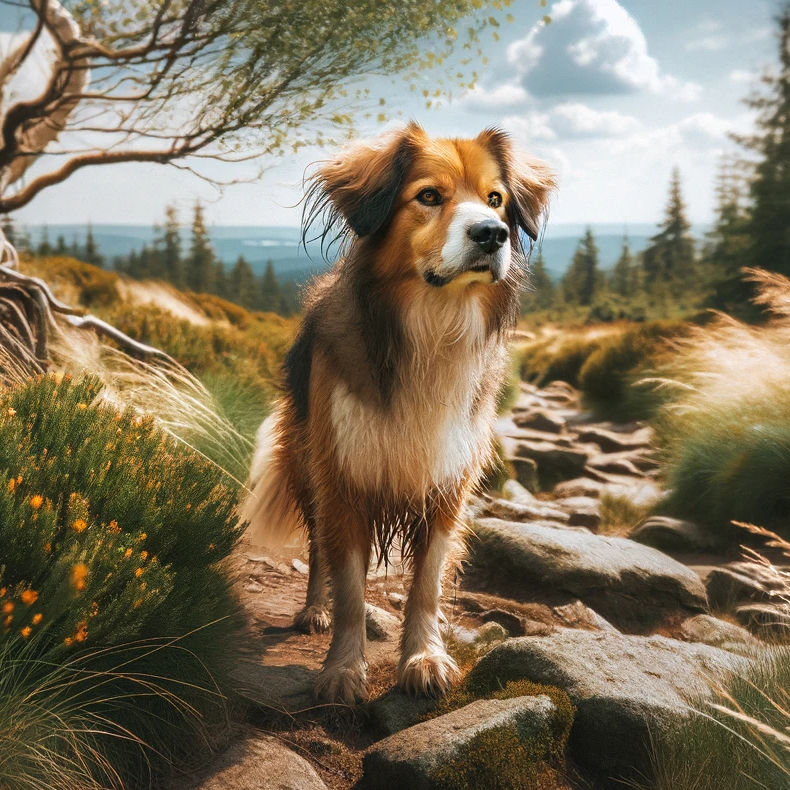
\includegraphics[height=0.5\textheight]{dog}
		
\includegraphics[height=0.5\textheight]{cat}
		\caption{What define the images?}
	\end{figure}
	\pause
	\begin{itemize}
		\item Examples can be defined by high level features.
		\item We will call to those features \textbf{code}
%		\item We will enter into deep generative modeling.
	\end{itemize}
\end{frame}


\begin{frame}
	\frametitle{Applications of generative modeling}
\begin{center}
	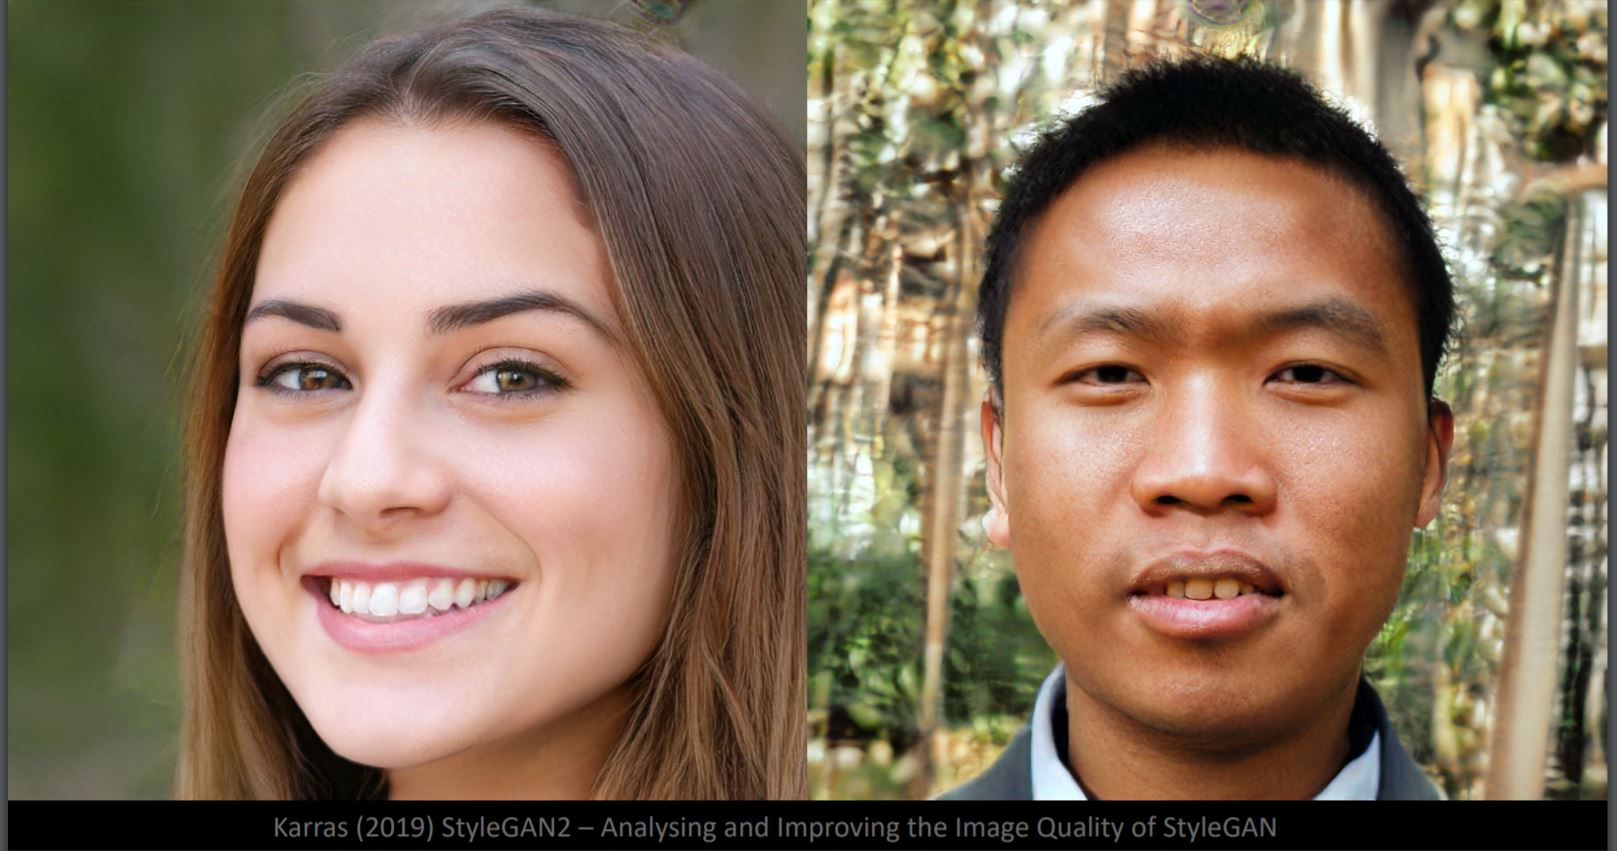
\includegraphics[height=0.8\textheight]{1_faces_gen}
\end{center}
\end{frame}


\section{Autoencoders}

% --- CONTEXT: UNSUPERVISED MODELS ---
\begin{frame}
	\frametitle{Unsupervised learning}
    %\framesubtitle{Context}
	\begin{itemize}
		\item Goal: learn structure from \textbf{unlabeled} data.
		\begin{center}
			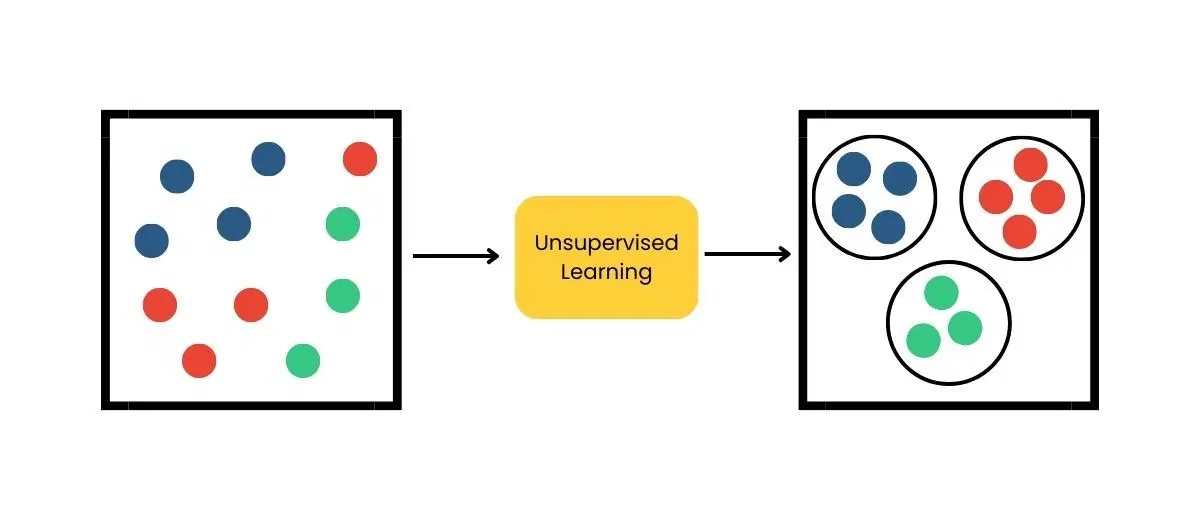
\includegraphics[height=0.6\textheight]{unsup}
		\end{center}
%		\item Families:
%		\begin{itemize}
%			\item \textbf{Autoencoders (AE):} reconstruction-based representation learning.
%			\item \textbf{Convolutional AE (CAE):} image-specific AEs with spatial priors.
%			\item \textbf{Variational AE (VAE):} probabilistic latent variables for generation.
		%\end{itemize}
		\item Benefits: denoising, compression, pretraining, and generative modeling.
	\end{itemize}
\end{frame}


% --- TAXONOMY ---

\begin{frame}
\frametitle{Autoencoders}
\begin{figure}
	\centering
	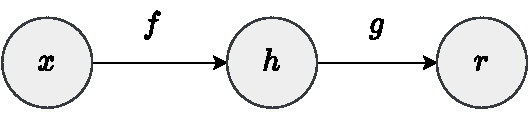
\includegraphics[height=0.2\textheight]{autoencoder.drawio}
%	\caption{}
	\label{fig:autoencoder}
\end{figure}

\begin{itemize}
	\item An autoencoder is a neural network that is trained to try to copy its input to its output
	\begin{equation}
		h = f(x)
	\end{equation}, $h$ is an embedding that describes the input, where $f$ is an encoder function.
	\begin{equation}
		r = g(h)
	\end{equation} is a reconstruction of the input, where $g$ is a decoder function. We expect that:
    $$r \simeq x$$
\end{itemize}
\end{frame}


\begin{frame}
\frametitle{Autoencoders}
\framesubtitle{Notation}
\begin{figure}
	\centering
	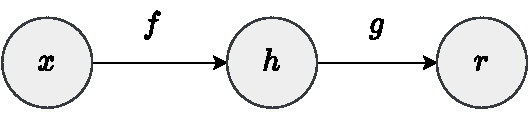
\includegraphics[height=0.2\textheight]{autoencoder.drawio}
%	\caption{}
	\label{fig:autoencoder}
\end{figure}

\begin{itemize}
        \item An autoencoder with parameters is written as:
        \begin{equation}
            r = g_{\phi}(f_{\theta}(x))
        \end{equation} where $\theta$ are the encoder parameters and $\phi$ are the decoder parameters.
        \item Condensed representation:
        \begin{equation}
            r = \Phi_{\theta,\phi} (x)
        \end{equation}
\end{itemize}
\end{frame}


\begin{frame}
	\frametitle{Training}
	The learning process minimizes the reconstruction loss:
	\begin{equation}
		\min \mathcal{L}(x, g(f(x))) 
	\end{equation} e.g.
\begin{equation}
   \mathcal{L}(x, r) = \sum_{i} (x_i - r_i)^2
\end{equation}
\end{frame}


\begin{frame}
	\frametitle{Undercomplete autoencoders}
	\framesubtitle{Bottleneck}
	\begin{columns}[T,onlytextwidth]
		\column{0.5\textwidth}
		\begin{itemize}
            \item The embedding is smaller than input.
			\item Learning useful features in the bottleneck:
			$$|x| = |r|$$
			\[
			|h| \ll |x|
			\]
			\item The lantent space, $\mathcal{H}$, captures the most relevant structure of $\mathcal{X}$.
		\end{itemize}
		\column{0.5\textwidth}
		\begin{center}
			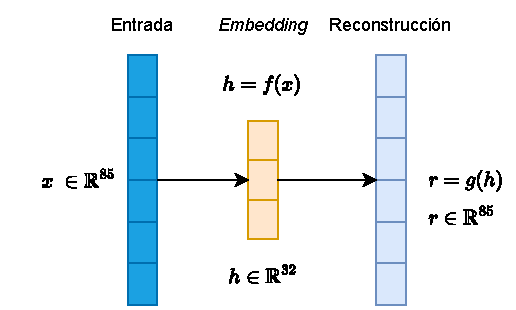
\includegraphics[height=0.5\textheight]{undercomplete}
		\end{center}
	\end{columns}
\end{frame}



\begin{frame}
	\frametitle{Dimensionality reduction \footnote{\scriptsize Hinton and Ruslan "Reducing the dimensionality of data with neural networks." science 313.5786 (2006): 504-507.}}
	\begin{columns}
		\begin{column}{0.4\textwidth}
			\centering
			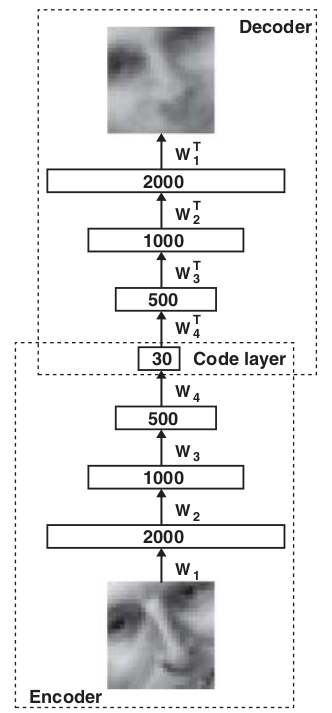
\includegraphics[width=\linewidth, height=0.8\textheight, keepaspectratio]{hinton2006}
		\end{column}
		\begin{column}{0.6\textwidth}
			\centering
			\begin{itemize}
				\item \textbf{Cross-Entropy Error for Logistic Output Units} (Binary/Continuous data in range [0, 1]).
       			$$-\sum_{i}p_{i}\log\hat{p}_{i}-\sum_{i}(1-p_{i})\log(1-\hat{p}_{i})$$
				\item This function was used for the synthetic "curves" data and the MNIST handwritten digit data, where pixel intensities are between 0 and 1.
			\end{itemize}
			
		\end{column}
	\end{columns}
\end{frame}


\begin{frame}{}
	
\begin{center}
	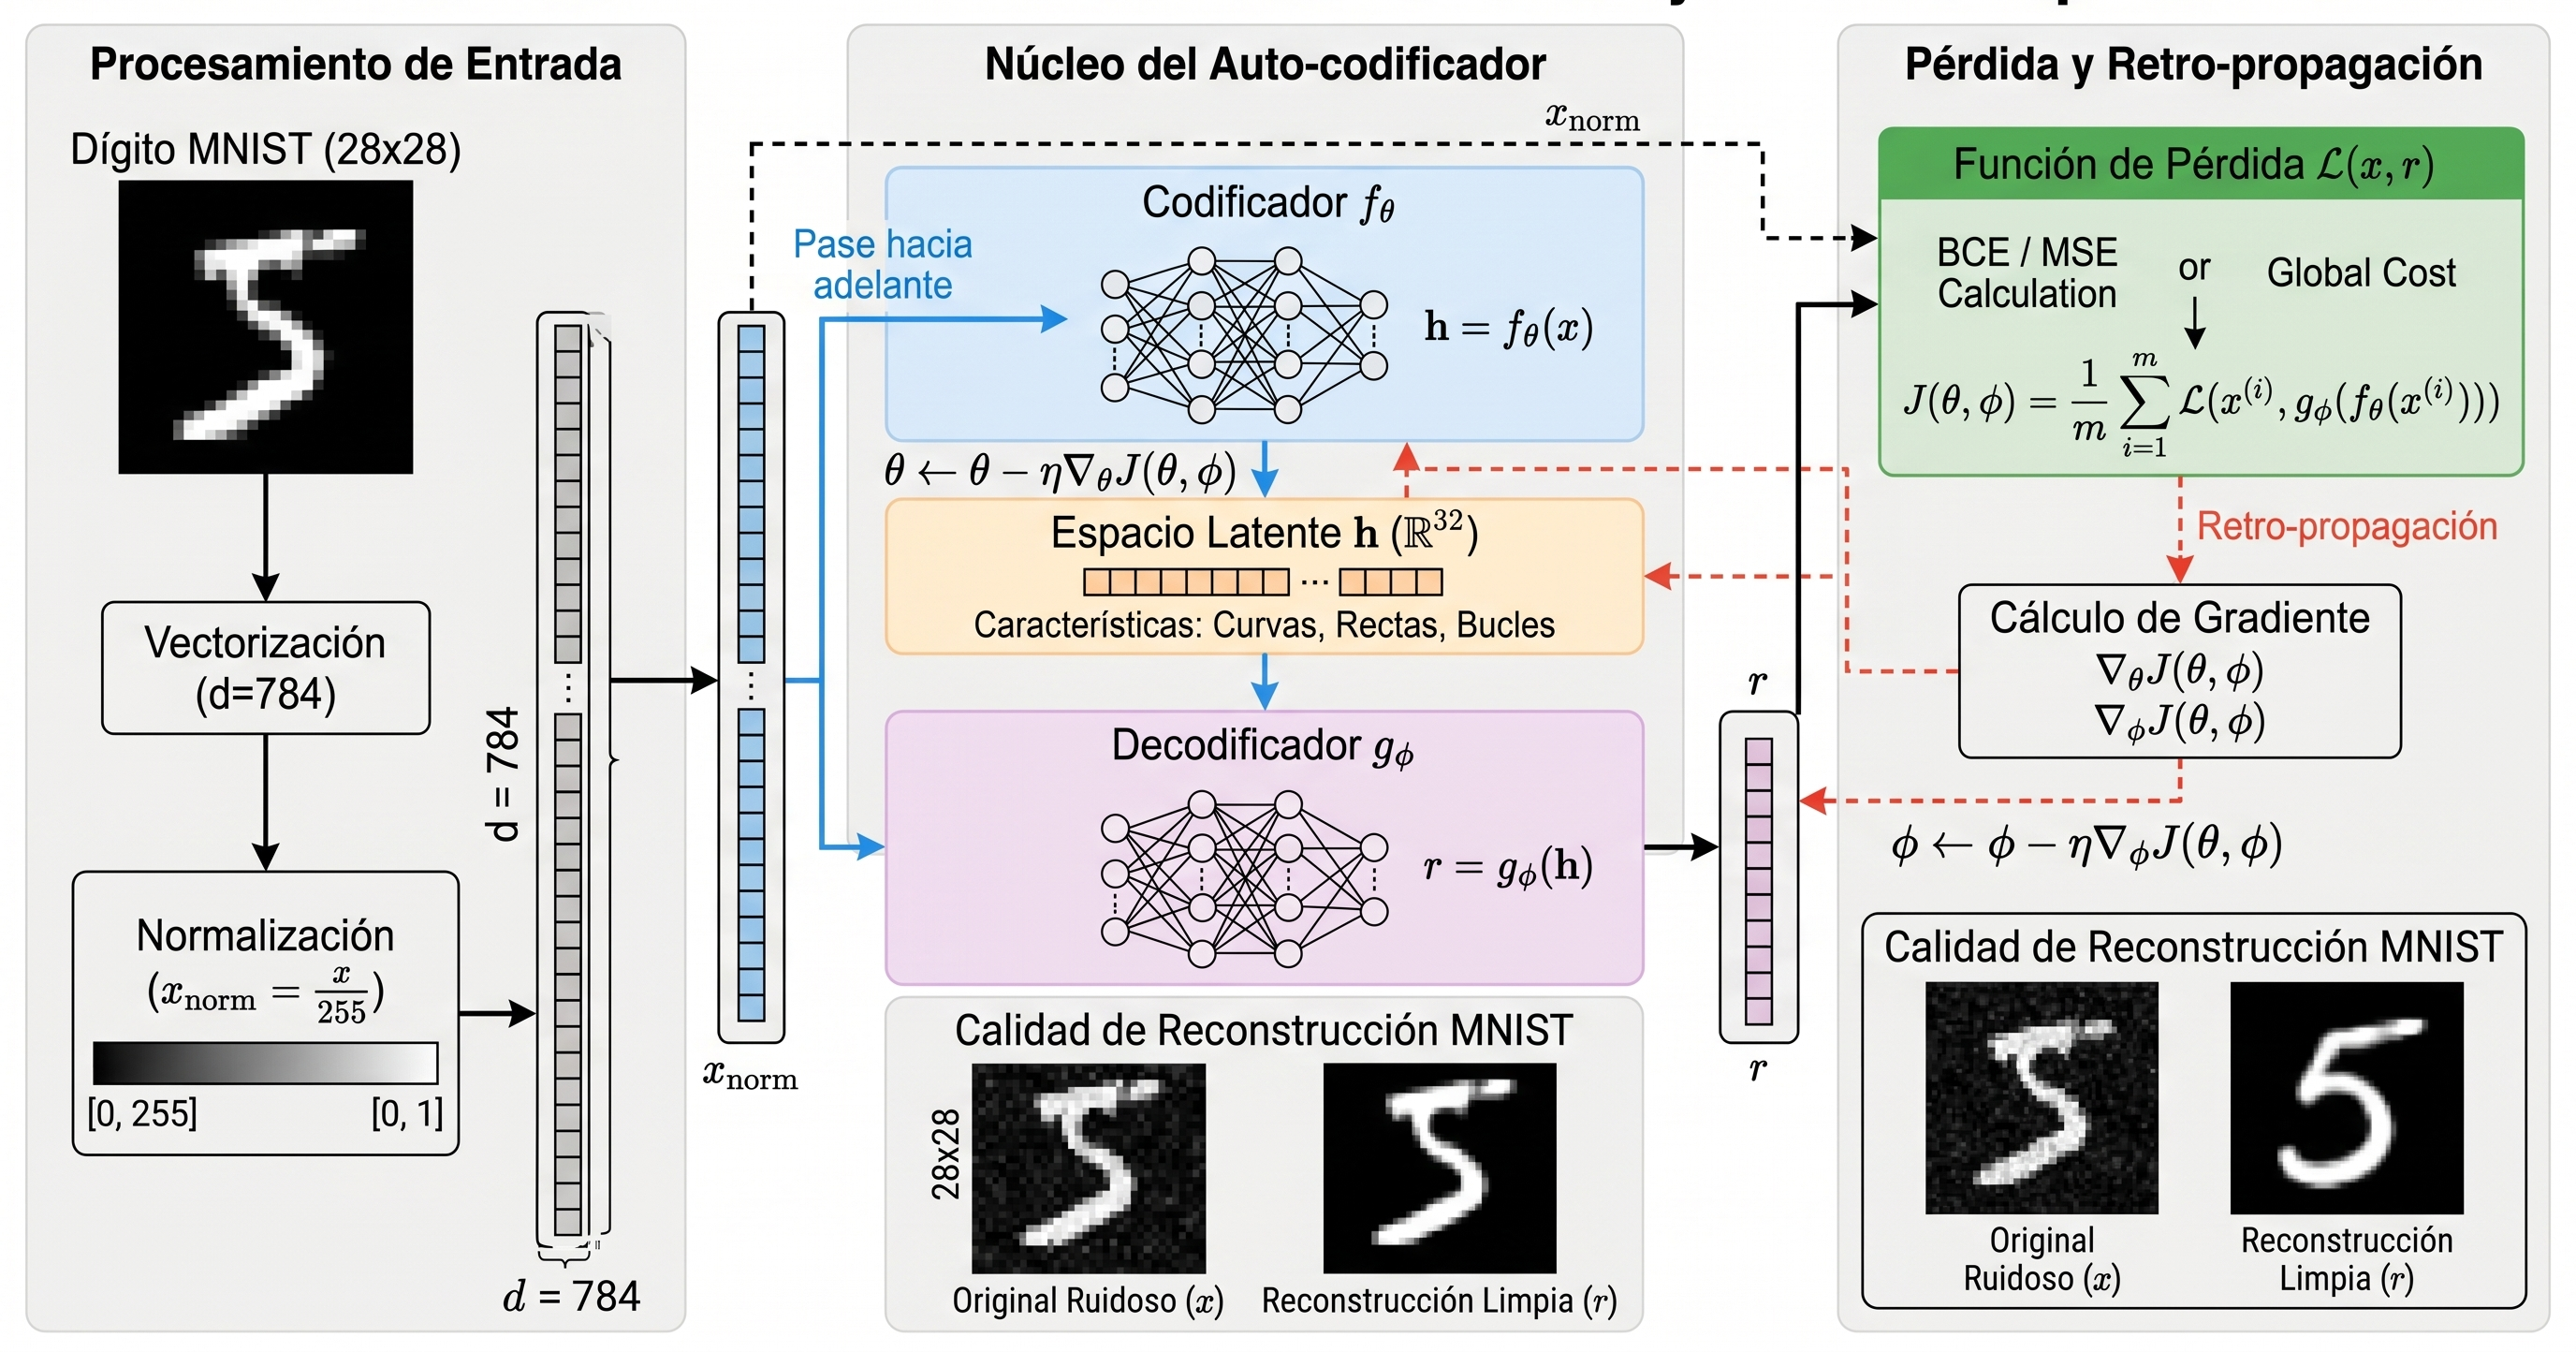
\includegraphics[height=0.9\textheight]{train_fase}
\end{center}
\end{frame}


\begin{frame}{Comparison against PCA}
    \begin{figure}
        \centering
        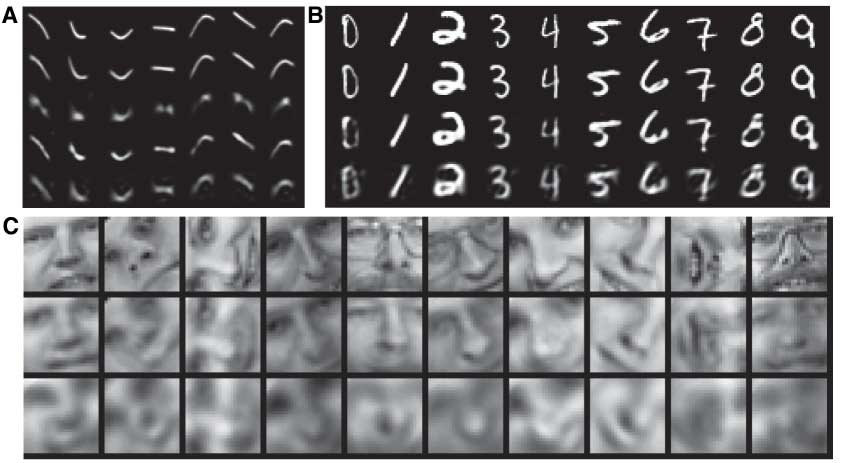
\includegraphics[height=0.7\textheight]{results_ autoencoder.png}
        \caption{Rows: Original, autoencoder, logistic PCA 6, log PCA 18, standard PCA.}    
        \label{fig:placeholder}
    \end{figure}
\end{frame}

\begin{frame}{Comparison against PCA}
    \begin{figure}
        \centering
        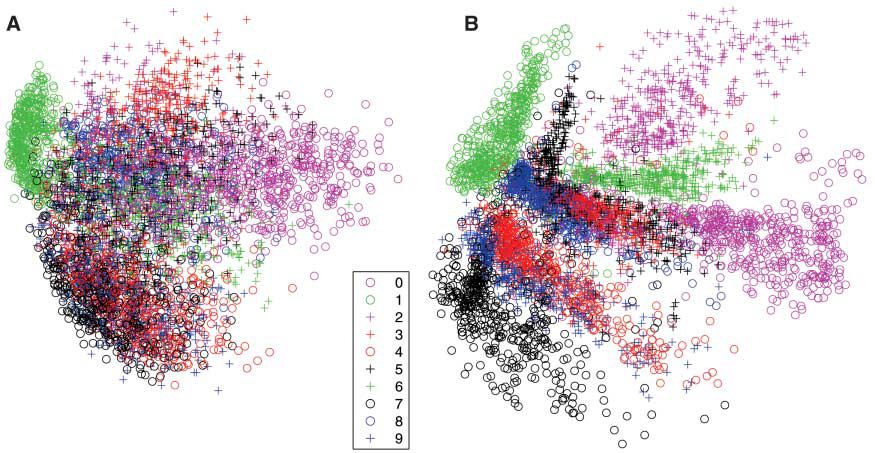
\includegraphics[height=0.7\textheight]{digits.png}
        \caption{PCA vs Autoencoder for MNIST digits.}
        \label{fig:placeholder}
    \end{figure}
\end{frame}

\begin{frame}
	\frametitle{Undercomplete autoencoders}
	\framesubtitle{Classification application}
	\begin{itemize}
		\item Labeled data is scarce and small amounts of data can lead to overfit.
		\item Huge amount of unlabeled data.
	\end{itemize}
	\begin{figure}
		\centering
		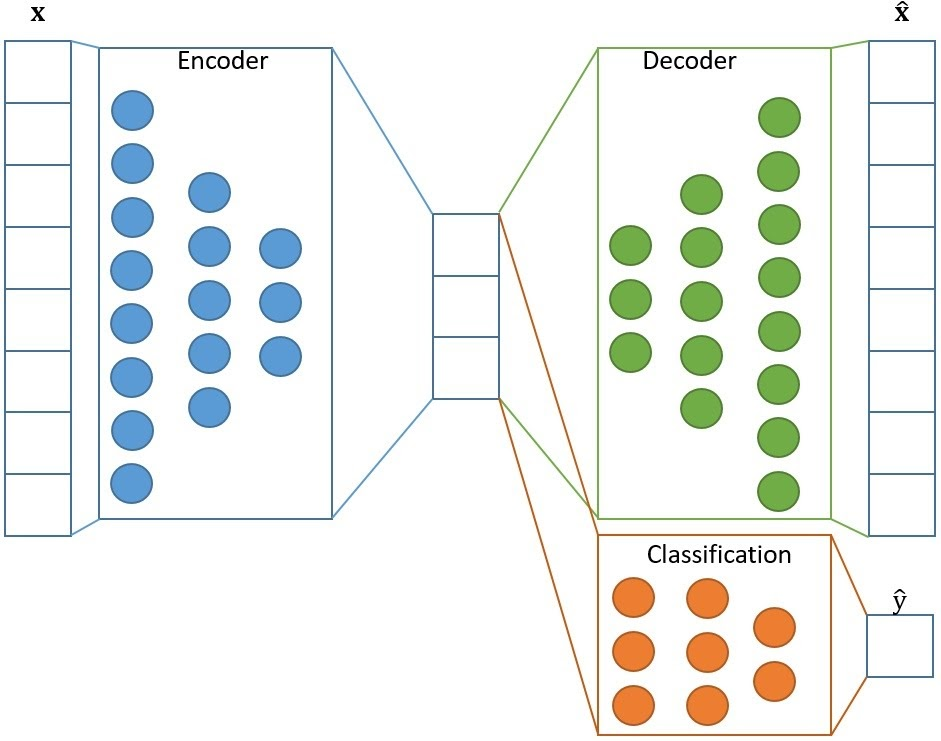
\includegraphics[height=0.5\textheight]{classification.jpg}	%\caption{}
		\label{fig:embedding}
        \caption{Example of the use of an autoencoder to solve classification tasks\footnote{\scriptsize Bank, D., Koenigstein, N., \& Giryes, R. (2023). Autoencoders. Machine learning for data science handbook, 353-374.}.}
	\end{figure}
\end{frame}



\section{Convolutional autoencoders}


\begin{frame}
	\frametitle{Convolutional autoencoders}
	\begin{itemize}
		\item Replace dense layers with conv / (transposed) conv.
		\item Preserves locality; better image reconstructions.
	\end{itemize}
\end{frame}



% --- CONVOLUTIONAL AUTOENCODERS ---
\begin{frame}
	\frametitle{Convolutional Autoencoders (CAE)\footnote{Masci, Jonathan, et al. "Stacked convolutional auto-encoders for hierarchical feature extraction." International conference on artificial neural networks. Berlin, Heidelberg: Springer Berlin Heidelberg, 2011.}}
	\begin{columns}[T,onlytextwidth]
		\column{0.45\textwidth}
		\begin{itemize}
			\item \textbf{Encoder}:\\ Conv $\rightarrow \sigma(h) \rightarrow$ Pool.
			\item \textbf{Code}:\\ small $H'\!\times\!W'\!\times\!C'$ feature tensor.
			\item \textbf{Decoder}:\\ Transposed Conv / UpSampling.
			\item \textbf{Why better for images?} Weight sharing \& locality priors.
			\item Typical losses: $\ell_2$ (pixel MSE), $\ell_1$, SSIM, or hybrid.
		\end{itemize}
		\column{0.55\textwidth}
		\begin{figure}
			\centering
			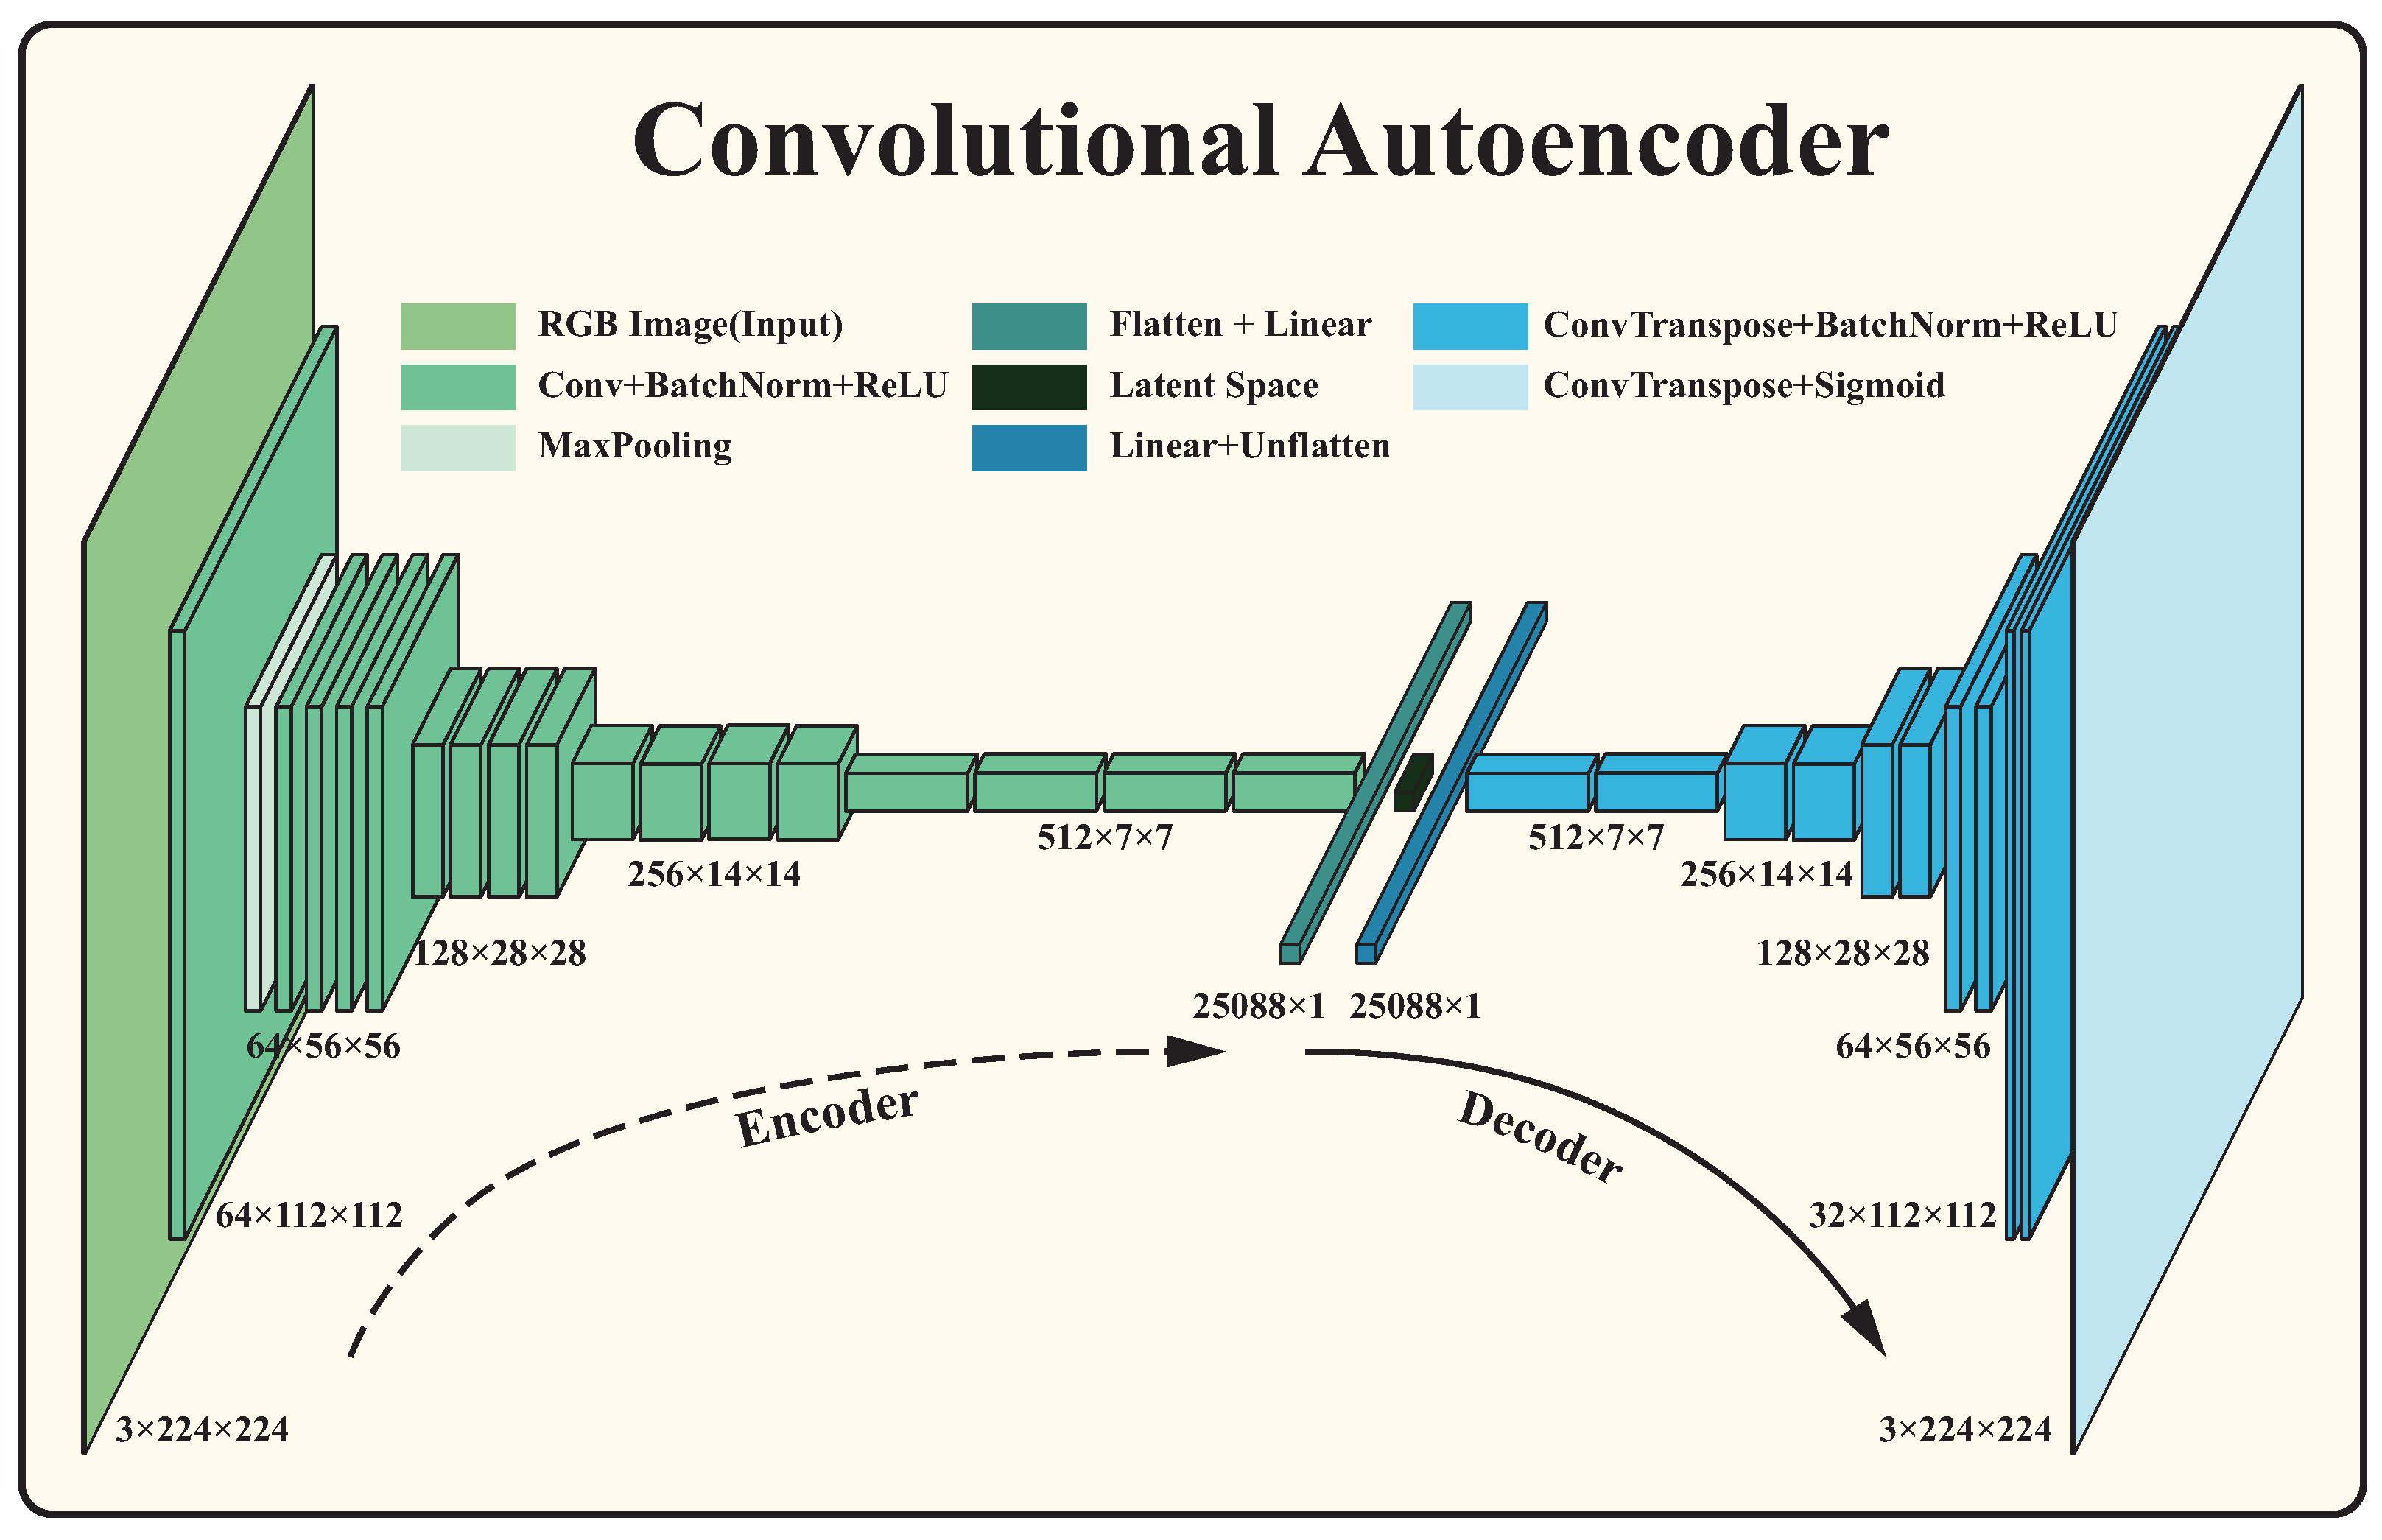
\includegraphics[height=0.55\textheight]{buildings-14-02828-g002}
			\caption{\small CAE: conv bottleneck preserves spatial structure }
		\end{figure}
	\end{columns}
\end{frame}


% --- LATENT SPACE OPERATIONS ---
\begin{frame}
	\frametitle{Latent Space: Interpolation \& Arithmetic}
	\begin{itemize}
		\item \textbf{Linear interpolation}:
		\[
		z_\alpha = (1-\alpha)z_1 + \alpha z_2,\ \ \alpha\in[0,1]
		\]
		\item Decode $g_\phi(z_\alpha)$ to visualize smooth morphs (e.g., dog $\rightarrow$ bird).
	\end{itemize}
\end{frame}


\begin{frame}
	\frametitle{Interpolating}
	\framesubtitle{Image space}
	\begin{center}
		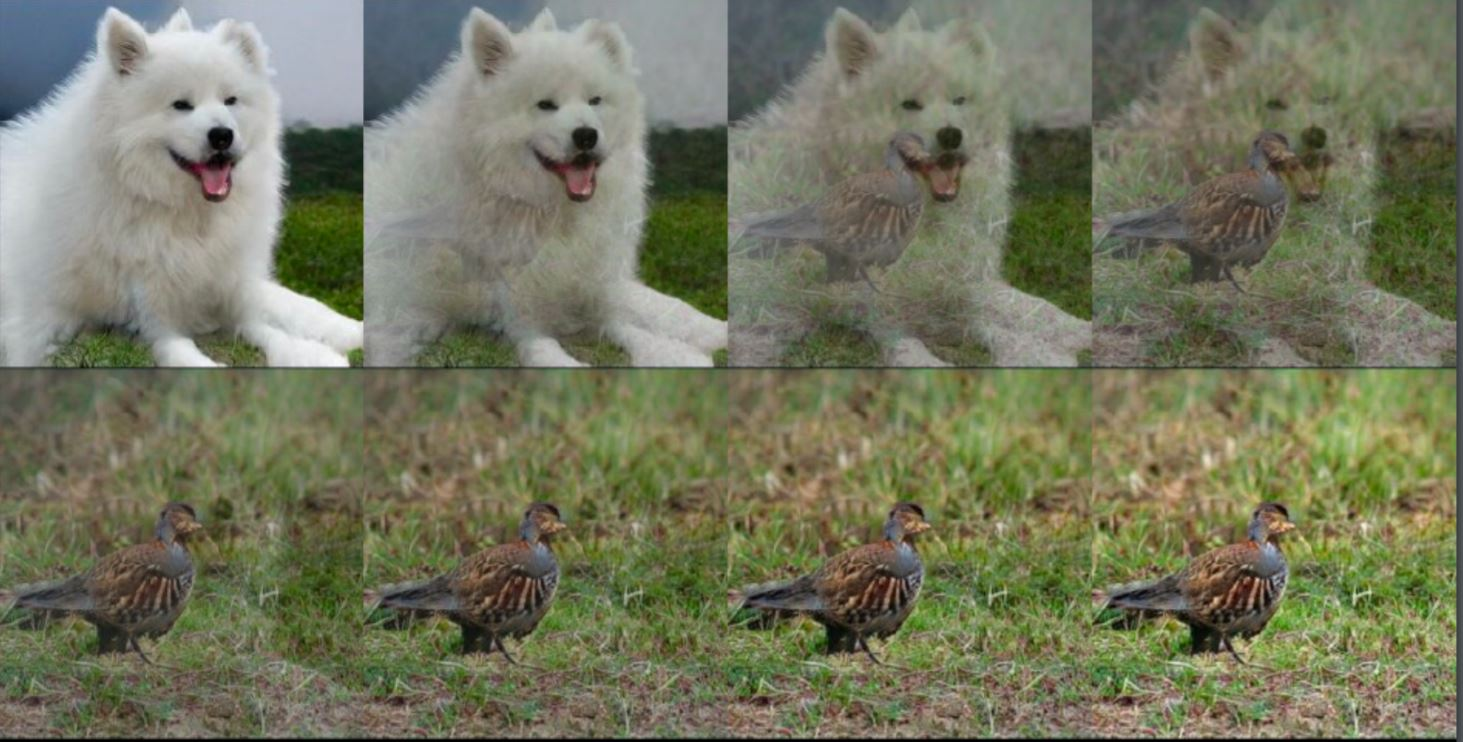
\includegraphics[height=0.75\textheight]{3_dog2bird}
	\end{center}
\end{frame}


\begin{frame}
	\frametitle{Interpolating}
	\framesubtitle{Latent space}
	\begin{center}
		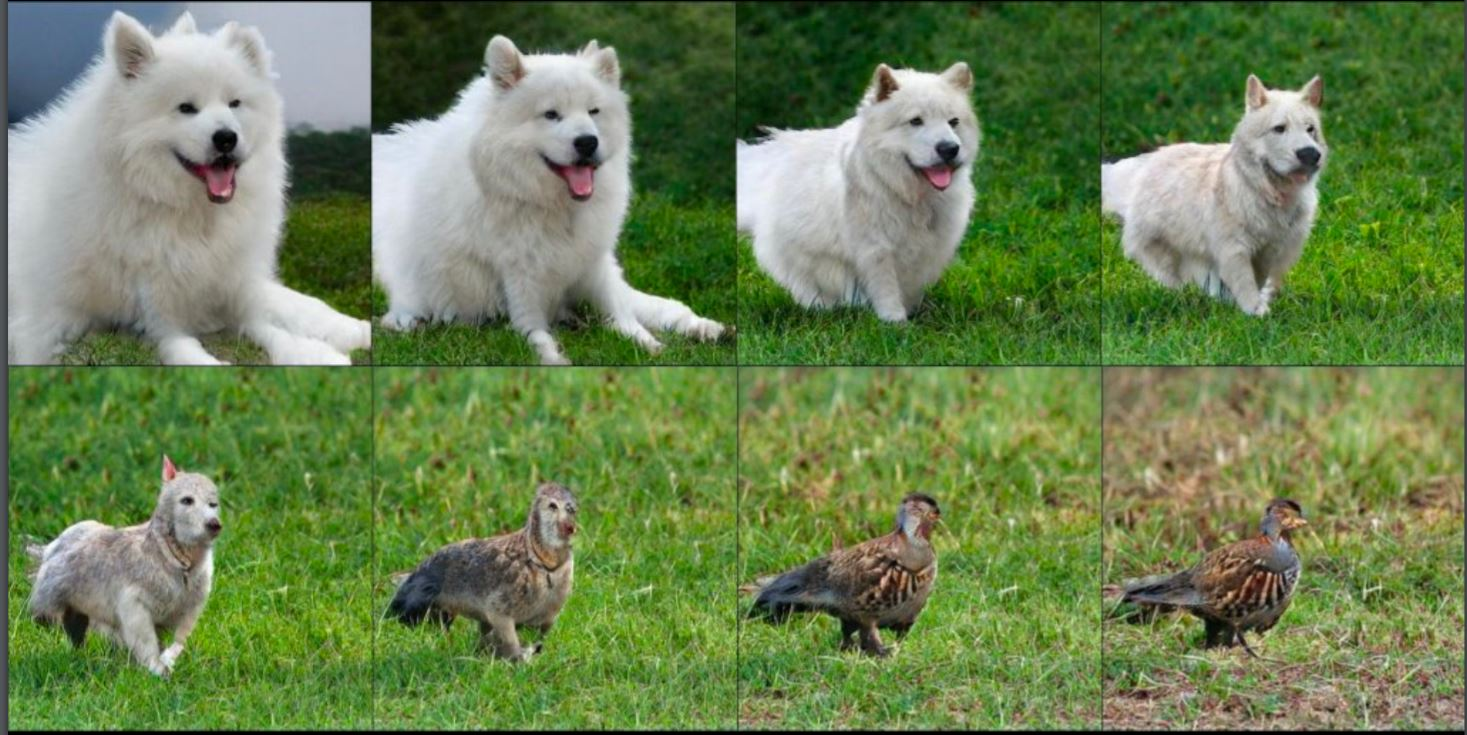
\includegraphics[height=0.75\textheight]{4_model_d2b}
	\end{center}
\end{frame}


% --- LATENT SPACE OPERATIONS ---
\begin{frame}
	\frametitle{Latent Space: Interpolation \& Arithmetic}
	\begin{columns}[T,onlytextwidth]
		\column{0.52\textwidth}
		\begin{itemize}
			\item \textbf{Linear interpolation}:
			\[
			z_\alpha = (1-\alpha)z_1 + \alpha z_2,\ \ \alpha\in[0,1]
			\]
			\item Decode $g_\phi(z_\alpha)$ to visualize smooth morphs (e.g., dog $\rightarrow$ bird).
			\item \textbf{Attribute vectors}: $z_{\text{smile}} - z_{\text{neutral}}$; add to new $z$.
		\end{itemize}
		\column{0.44\textwidth}
		\begin{figure}
			\centering
			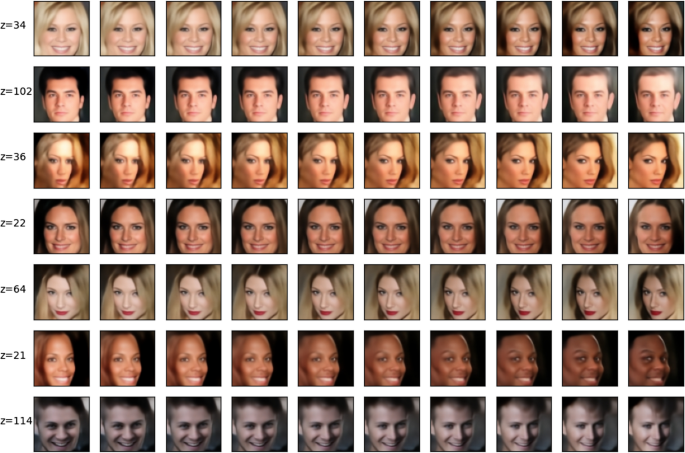
\includegraphics[height=0.5\textheight]{521_2022_7890_Fig6_HTML}
			\caption{\small Smooth changes along semantic directions}
		\end{figure}
	\end{columns}
\end{frame}


\begin{frame}
	\frametitle{Transformations in Latent Space}
	\begin{center}
		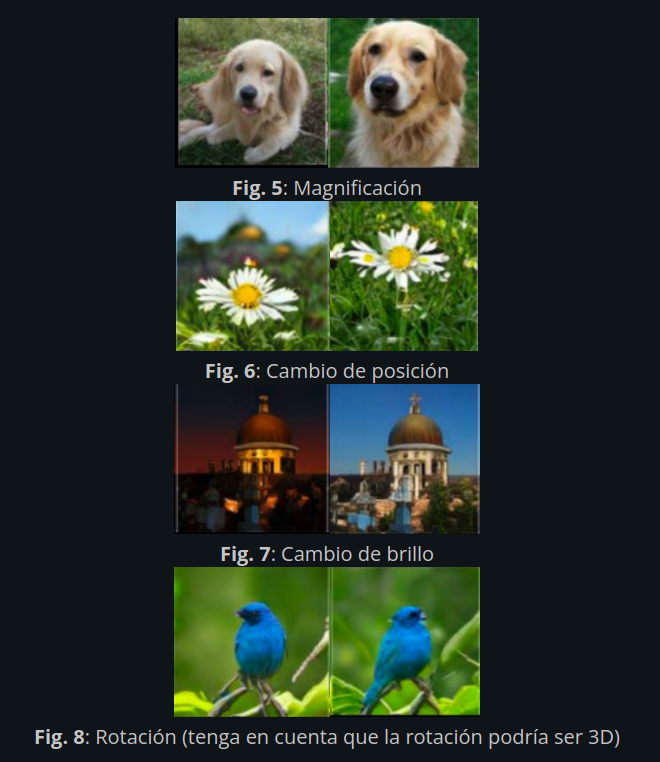
\includegraphics[height=0.85\textheight]{Transf_ls.png}
	\end{center}
\end{frame}


\section{Denoising autoencoders}


\begin{frame}
	\frametitle{Denoising autoencoder}
	%\framesubtitle{Superesolution}
    \begin{itemize}
     \item Denoising autoencoders
\begin{equation}
\min \mathcal{L}(x, g(f(\tilde{x})))
\end{equation} where $\tilde{x}$ is a copy of $x$ that has been corrupted by some noise. i.e. $$ p(\tilde{x}|x)$$
\item Noise models: Gaussian, masking (salt \& pepper), dropout-like corruption.
    \end{itemize}
\end{frame}

\begin{frame}
	\frametitle{Denoising autoencoder}
	\framesubtitle{Superesolution example}
    \begin{itemize}
     \item Task: To recover a high resolution image from a low resolution image.
     \begin{equation}
         r = g(f(\tilde{x}))
     \end{equation} where $x$ is the original image, $\tilde{x}$ is the low resolution image and $r$ the recovered image.
    \end{itemize}
    	\begin{center}
		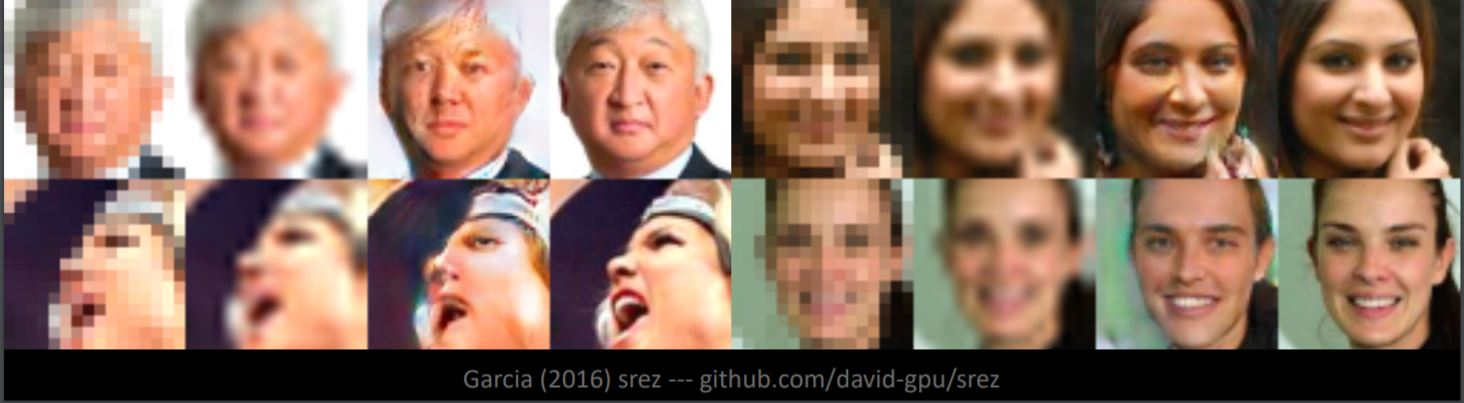
\includegraphics[height=0.45\textheight]{9_reconstruct}
	\end{center}
\end{frame}


\begin{frame}
	\frametitle{Denoising autoencoders}
	%\framesubtitle{Denoising autoencoders}
	\begin{itemize}
		\item Receives a corrupted data point as input and it is trained to predict the original.
        \item \textbf{Training}: sample $\tilde x \!\sim\! q(\tilde x|x)$; encode--decode; penalize $L(x,r)$.
        \begin{center}
        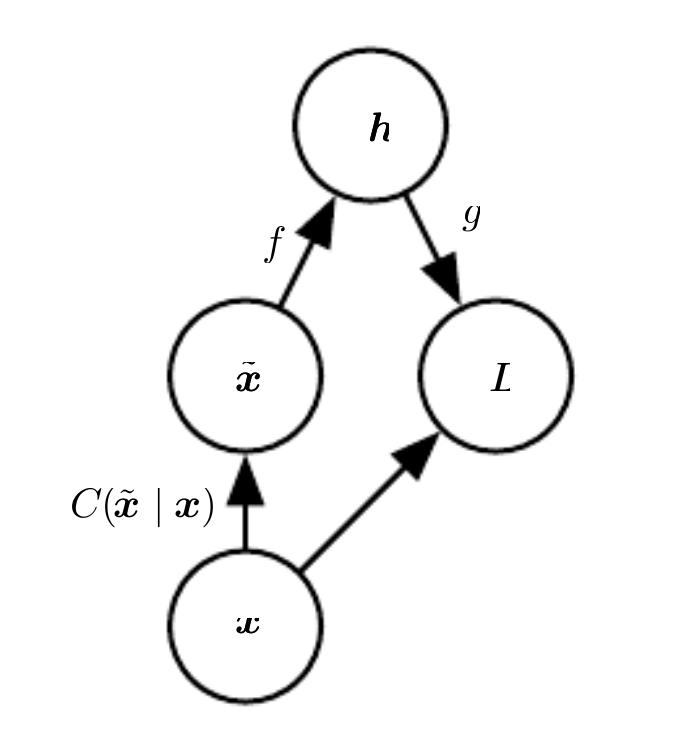
\includegraphics[height=0.5\textheight]{datrain}    
        \end{center}
        
		\item \textbf{Intuition}: forces encoder to learn \emph{stable} features that survive corruption.
	\[
	\tilde x = x + \epsilon,\ \epsilon \sim \mathcal{N}(0,\sigma^2 I)
	\quad\Rightarrow\quad
	\min_{\theta,\phi}\ \mathbb{E}_{\tilde x}\ \|x - g(f(\tilde x))\|^2
	\]
	\end{itemize}
\centering

\end{frame}


\begin{frame}
%	\frametitle{Autoencoders}
%	\framesubtitle{Denoising autoencoders}
\begin{center}
	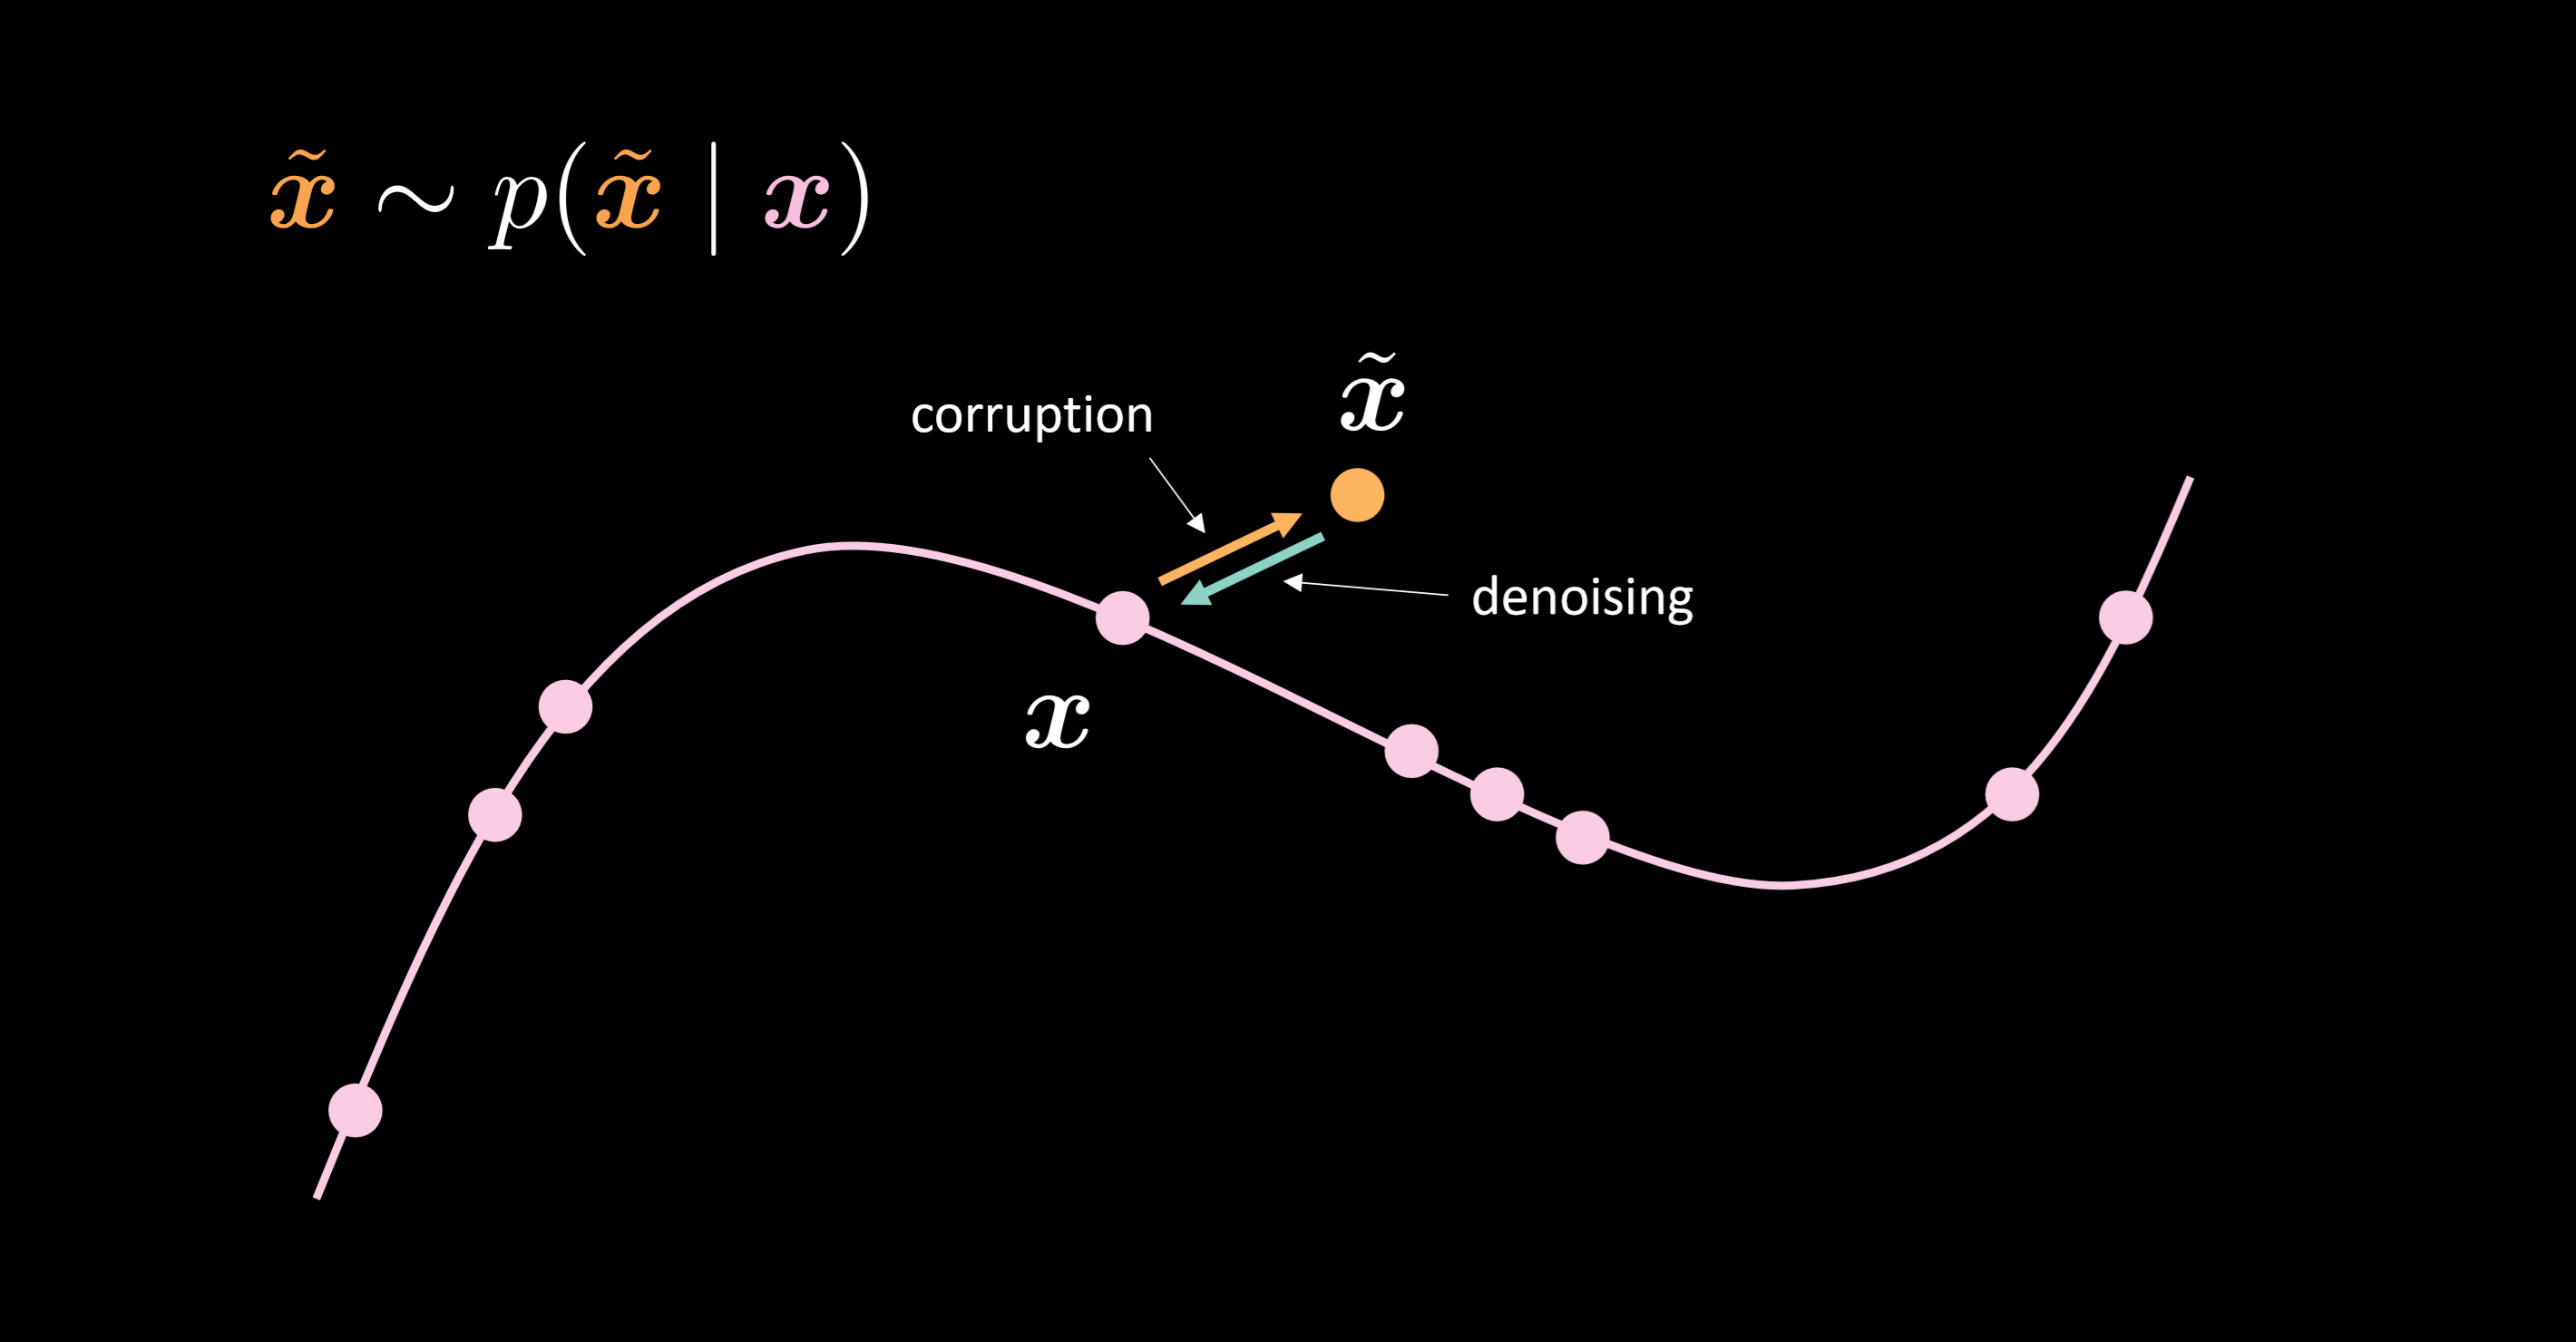
\includegraphics[height=0.9\textheight]{15_denoising_ae}
\end{center}
\end{frame}


%\begin{frame}
%\frametitle{Autoencoders}
%\framesubtitle{Denoising autoencoders}
%\begin{center}
%	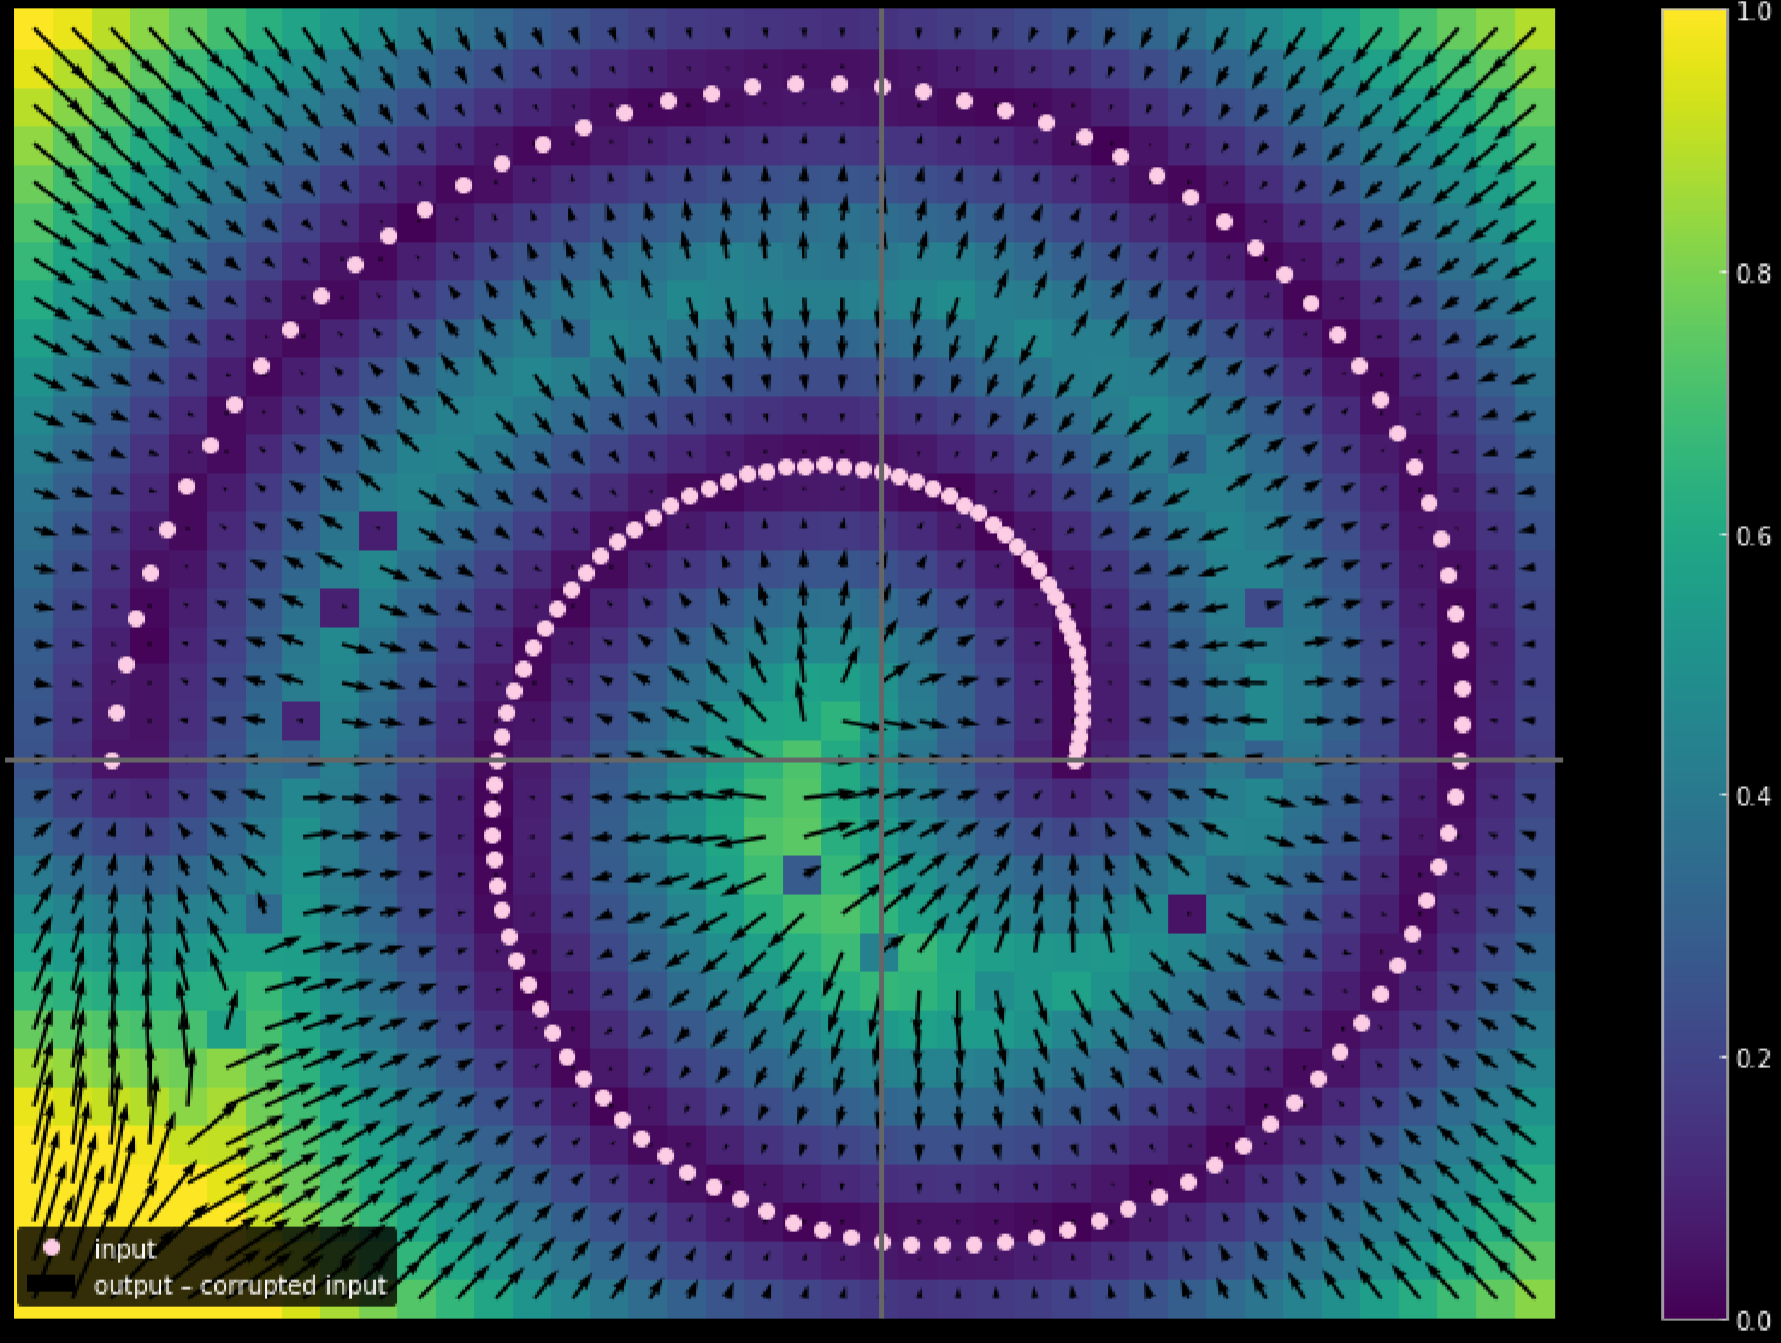
\includegraphics[height=0.8\textheight]{17_distance}
%\end{center}
%\end{frame}


\begin{frame}{Regularized autoencoders}
	\framesubtitle{Notation and organization}
	\begin{itemize}
		\item Regularized autoencoders try to avoid the identity function inside the autoencoder.
		\begin{equation}
			\begin{pmatrix}
				h_1 \\
				h_2 \\
				h_3
			\end{pmatrix}
			=
			\begin{pmatrix}
				1 & 0 & 0 \\
				0 & 1 & 0 \\
				0 & 0 & 1
			\end{pmatrix}
			\begin{pmatrix}
				x_1 \\
				x_2 \\
				x_3
			\end{pmatrix}
		\end{equation}
		\item They add a term to the loss function:
		\begin{equation}
			\mathcal{L}(x,r) = E(x,r) + \Omega(c)
		\end{equation}
		where $E(x,r)$ is the standard reconstruction error and
		$\mathbf{\Omega}(c)$ is a regularization term.
	\end{itemize}
\end{frame}


\section{Regularized autoencoders}


\begin{frame}{Regularized autoencoders}
	\framesubtitle{Sparse Autoencoders}
	\begin{columns}
		\begin{column}{0.5\textwidth}
			\begin{itemize}
				\item Sparse Autoencoders encourage near-zero activations in the code layer $h$.
				\begin{equation}
					\min \mathcal{L}(x,r) = E(x,r) + \Omega(h)
				\end{equation}
				\item $\mathbf{\Omega(h)}$ is a sparsity penalty on the code layer $h$. This penalty enforces that only a small number of hidden units are active for any given input.
			\end{itemize}
		\end{column}
		\begin{column}{0.5\textwidth}
			\centering
			\begin{figure}
				\centering
				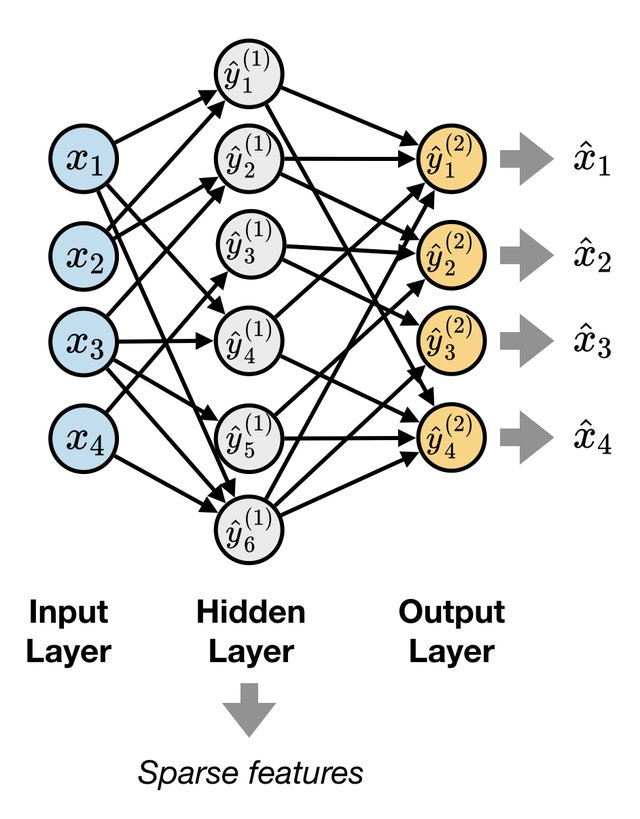
\includegraphics[width=\linewidth, height=0.6\textheight, keepaspectratio]{sparse.jpg}
				\caption{Example of a sparse autoencoder\footnote{\scriptsize Dutta, S., Bai, Z., Jeong, H., Low, T. M., \& Grover, P. (2018, June). A unified coded deep neural network training strategy based on generalized polydot codes. In 2018 IEEE International Symposium on Information Theory (ISIT) (pp. 1585-1589). IEEE.}.}
			\end{figure}
		\end{column}
	\end{columns}
\end{frame}


\begin{frame}{Regularized autoencoders}
	\framesubtitle{Contractive Autoencoders}
	\begin{columns}
		\begin{column}{0.5\textwidth}
			\begin{itemize}
				\item They are designed to learn a representation ($\mathbf{h}$) that is \textbf{robust to small variations} in the input data ($\mathbf{x}$).
                \begin{equation}
                    \tilde{x} = T(x)
                \end{equation}
			\end{itemize}
		\end{column}
		
		\begin{column}{0.5\textwidth}
			\centering
    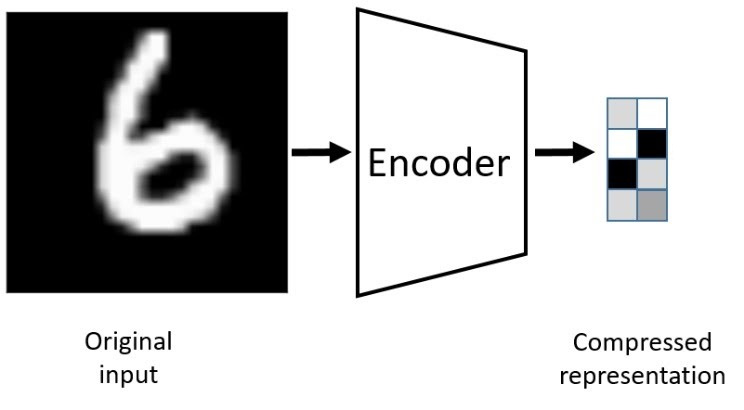
\includegraphics[height=0.4\textheight]{contractive_a.jpg} \\
    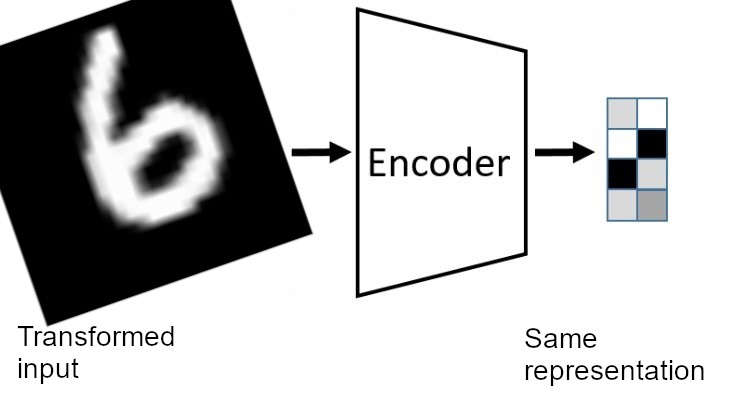
\includegraphics[height=0.4\textheight]{contractive_b.jpg}
		\end{column}
	\end{columns}
\end{frame} 


\begin{frame}{Regularized autoencoders}
	\framesubtitle{Contractive Autoencoders}    
	\begin{itemize}
        \item The learned features are forced to be \textbf{locally invariant} to input perturbations.
        \item The overall objective function to minimize is:
			$$ \mathcal{L}(x,g(f(\mathbf{\tilde{x}}))) = E(x, g(f(\mathbf{\tilde{x}}))) + \Omega(x) $$
        \item Regularization Term, $\Omega(x)$:
			The penalty term is the squared Frobenius norm of the Jacobian matrix of the encoder's output with respect to the input:
			$$ \Omega(x) = \lambda \left\| \frac{\partial f(\mathbf{x})}{\partial \mathbf{x}} \right\|_F^2 $$ where $f(\mathbf{x})$ is the encoder function, $\mathbf{\lambda}$ is the regularization coefficient, $\Omega(x)$ forces the partial derivatives to be small, thus "contracting" the input manifold.
    \end{itemize}
\end{frame}


\begin{frame}
	\frametitle{Contractive Autoencoders}
    \framesubtitle{Applications}
	\begin{itemize}
		\item \textbf{Robust Feature Extraction}: Scenarios where the input data contains noise or slight variations (e.g., small shifts or rotations in images), as the model is penalized for changing its embedded when the input changes slightly.
		\item \textbf{Learning Stable Features}: By enforcing local invariance, CAEs learn features that are stable, making them valuable for tasks like transfer learning.
		\item \textbf{Improving Deep Network Performance}: The features learned by a CAE can be used to initialize the weights of deeper supervised networks, providing a robust starting point that often leads to faster convergence and better final performance compared to random initialization.
	\end{itemize}
	\centering
\end{frame}




\section{Variational autoencoders}


% --- VARIATIONAL AUTOENCODERS (INTRO) ---
\begin{frame}
	\frametitle{Variational Autoencoders (VAE)}
	\framesubtitle{From Deterministic Codes to Probabilistic Latents}
	\begin{itemize}
		\item \textbf{Latent variable model}: $z \sim p(z)=\mathcal{N}(0,I)$,\quad $x \sim p_\phi(x|z)$.
		\item \textbf{Encoder (inference)}: $q_\theta(z|x)=\mathcal{N}\!\big(\mu(x),\mathrm{diag}(\sigma^2(x))\big)$.
		\item \textbf{Reparameterization}: $z=\mu(x)+\sigma(x)\odot\epsilon,\ \epsilon\sim\mathcal{N}(0,I)$.
	\end{itemize}
	\[
	\mathcal{L}_{\text{VAE}}(x)
	= \underbrace{\mathbb{E}_{q_\theta(z|x)}[-\log p_\phi(x|z)]}_{\text{reconstruction}}
	+ \beta\,\underbrace{D_{KL}\!\big(q_\theta(z|x)\,\|\,p(z)\big)}_{\text{regularization}}
	\]
	\begin{itemize}
		\item \textbf{$\beta$-VAE}: increase $\beta$ for more disentangled factors (trade-off with recon).
	\end{itemize}
\end{frame}


\begin{frame}
\begin{figure}
	\centering
	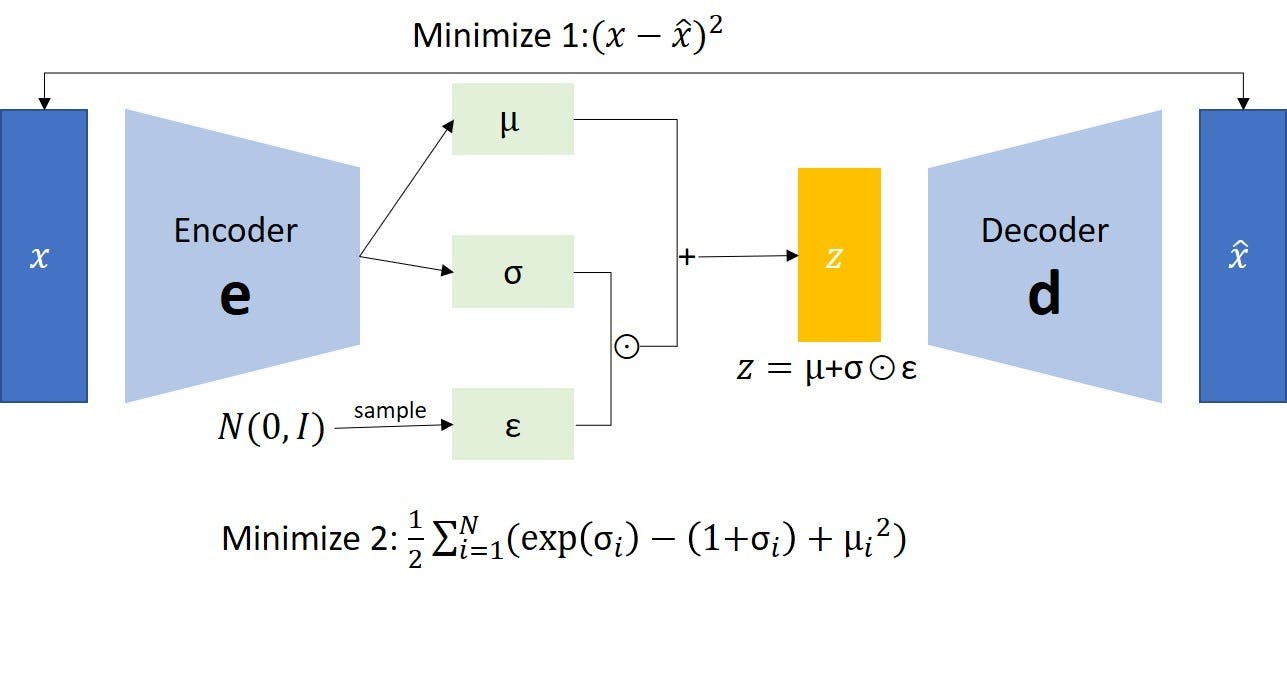
\includegraphics[width=0.7\linewidth]{1_r1R0cxCnErWgE0P4Q-hI0Q}
	\caption{Variational autoencoder illustration}
	\label{fig:1r1r0cxcnerwge0p4q-hi0q}
\end{figure}
\end{frame}



\begin{frame}
\frametitle{Summary}
	\begin{tikzpicture}[
		edge from parent/.style={draw, -{Stealth[scale=1.2]}, thick},
		level 1/.style={sibling distance=5cm, level distance=2cm},
		level 2/.style={sibling distance=4.5cm, level distance=2.5cm},
		every node/.style={rectangle, draw, rounded corners, fill=blue!5, 
			text width=3.5cm, align=center, font=\sffamily\small,
			inner sep=5pt}
		]
		
		% Nodo Raíz
		\node[fill=blue!20, font=\sffamily\bfseries] {Auto-codificador \\ $r = g_\phi(f_\theta(x))$}
		% Rama 1: Sub-completo
		child {
			node {Sub-completo \\ $|h| < |x|$}
		}
		% Rama 2: Eliminador de ruido
		child {
			node {Eliminador de Ruido \\ $\min \sum \mathcal{L}(x, g(f(\tilde{x})))$ \\ $\tilde{x} = \text{perturbación}$}
		}
		% Rama 3: Regularizados
		child {
			node[fill=green!10] {Regularizado \\ $\mathcal{L} = E(x,r) + \Omega(c)$}
			% Sub-ramas de Regularizados
			child {
				node {Disperso (Sparse) \\ $|h| > |x|$ \\ $\Omega(h) \to 0$}
				edge from parent node[left, draw=none, fill=none, xshift=-5pt] {}
			}
			child {
				node {Contractivo \\ $\tilde{x} = T(x)$ \\ $\Omega(h)$ penaliza derivadas}
				edge from parent node[right, draw=none, fill=none, xshift=5pt] {}
			}
		};
	\end{tikzpicture}
\end{frame}


% --- PRACTICAL NOTES ---
\begin{frame}
	\frametitle{Practical Notes}
	\begin{itemize}
		\item Normalize inputs (e.g., to $[0,1]$ or $[-1,1]$); monitor loss curves.
		\item Watch batch size vs.\ learning rate; too large LR can cause softmax/exp overflow.
		\item For images, prefer CAE or VAE with conv backbones for sharper reconstructions.
		\item Use validation recon error and sample quality (and SSIM/LPIPS) to compare models.
	\end{itemize}
\end{frame}







\begin{frame}
	\frametitle{References}
	\begin{itemize}
		\item Goodfellow, Ian, Yoshua Bengio, and Aaron Courville. Deep learning. MIT press, 2016.
		\item Bank, Dor, Noam Koenigstein, and Raja Giryes. "Autoencoders. arxiv." arXiv preprint arXiv:2003.05991 (2020): 2593-2613.
		\item NYU, Aprendizaje profundo,  \url{https://atcold.github.io/pytorch-Deep-Learning/es/week07/07-3/} 
	\end{itemize}
\end{frame}

%
%\begin{frame}
%	\frametitle{title}
%\end{frame}

\end{document}